\documentclass[../portafolio.tex]{subfiles}

% Solo agregue paquetes en el preámbulo de ../portafolio.tex

\begin{document}

\chapter{Ejemplo de derivada centrada}
\label{ch:ejemplo-derivadas}
\hfill \textbf{Fecha de la actividad:} 10 de septiembre de 2024

\medskip

En este capítulo, mostraremos cómo estimar el error de un esquema
numérico dado para estimar la derivada de una función real $f(x)$ de
argumento real $x$. En este caso, nos dan una regla de derivación como
sigue:
\begin{equation}
  \label{eq:der-centrada}
  f_\text{cen}'(x) = \frac{f(x+h/2) - f(x-h/2)}{h}\,,
\end{equation}
%
donde $h>0$ un número real positivo, el cual resulta ser un esquema de
derivada centrada de dos puntos. Así, estimaremos el error de
truncamiento utilizando expansiones en serie de Taylor de $f$. Luego,
estimaremos el error del esquema numérico debido a errores de redondeo
al evaluar $f$, para finalmente comparar la estimación de estos
errores en el caso en que $f(x)=\sqrt{x}$.

\medskip

\section{Estimación del error de truncamiento}
Si $h$ es lo suficientemente pequeño y si $f$ es suave y continua al rededor de $x$, entonces asumimos que la siguiente serie de Taylor existe:
\begin{equation}
  \label{eq:taylorhpm2}
  f(x\pm h/2) =
  f(x) \pm f'(x) \frac{h}{2} + f''(x) \frac{h^2}{2^2 \cdot 2!}
  \pm f'''(x) \frac{h^3}{2^3\cdot 3!}
  +  f^{(4)}(x) \frac{h^4}{2^4\cdot 4!} + \cdots
\end{equation}

Reemplazando \eqref{eq:taylorhpm2} en \eqref{eq:der-centrada}, encontramos:
\begin{align}
  \label{eq:deriv-trunc}
  f_\text{cen}'(x)
  &=
  f'(x) + f'''(x) \frac{h^2}{2^2\cdot 3!}
  +
    f^{(5)}(x) \frac{h^4}{2^4\cdot 5!} + \cdots \,, \nonumber \\
  &=
    f'(x) + f'''(\xi) \frac{h^2}{2^2\cdot 3!} \,,
\end{align}
%
donde hemos usado que, por el teorema del valor medio, se puede asegurar que existe un valor de $x-h/2\leq \xi x+h/2$ de modo que:
\begin{equation}
  \label{eq:trunca}
  f'''(\xi) \frac{h^2}{2^2\cdot 3!}
  =
  f'''(x) \frac{h^2}{2^2\cdot 3!}
  +
  f^{(5)}(x) \frac{h^4}{2^4\cdot 5!} + \cdots \,.
\end{equation}

Así, según la ecuación~\eqref{eq:deriv-trunc}, entonces existe un error del orden $O(h^2)$ entre la derivada analítica $f'(x)$ y su aproximación numérica según la ecuación~\eqref{eq:der-centrada}.

\section{Estimación del error de redondeo}
Cada vez que evaluamos $f$, es posible que estemos cometiendo algún error de redondeo. Por ejemplo, al evaluar $f(x\pm h/2)$, en realidad obtengamos una aproximación de esta función dada por
\begin{equation}
  \label{eq:approxf}
  \overline{f(x\pm h/2)} = f(x\pm h/2) (1 + \varepsilon_\pm)\,,
\end{equation}
%
donde $\varepsilon_\pm$ es un error que depende del signo que usemos en $x\pm h/2$. Por lo tanto, según las ecuaciones \eqref{eq:der-centrada} y \eqref{eq:deriv-trunc}, en realidad tenemos:
\begin{equation}
  \label{eq:der-err}
  f'(x) = \frac{\overline{f(x+h/2)} - \overline{f(x-h/2)}}{h} - f'''(\xi) \frac{h^2}{2^2\cdot 3!} \,.
\end{equation}

Usando \eqref{eq:approxf} en \eqref{eq:der-err} y reordenando, encontramos
\begin{align}
  \label{eq:der-err-ordenado}
  f'(x) - \frac{f(x+ h/2) - f(x- h/2)}{h} = \frac{f(x+ h/2)\varepsilon_+ - f(x- h/2) \varepsilon_-}{h} - f'''(\xi) \frac{h^2}{2^2\cdot 3!} \,.
\end{align}

El lado izquierdo de la ecuación~\eqref{eq:der-err-ordenado} es simplemente el error absoluto entre $f'(x)$ y su aproximación según \eqref{eq:der-centrada}. Luego,
\begin{align}
  E_\text{abs}
  &= \left|f'(x) - \frac{f(x+ h/2) - f(x- h/2)}{h}\right| \,, \label{eq:def-err-abs}
  \\
  &\leq
    \left|\frac{f(x+ h/2)\varepsilon_+}{h}\right| +
    \left|\frac{f(x- h/2)\varepsilon_-}{h}\right| +
    \left|f'''(\xi) \frac{h^2}{2^2\cdot 3!} \right| \,,
\end{align}
%
donde hemos usado la desigualdad triangular para separar varios términos. Si asumimos que $h$ es lo suficientemente pequeño, entonces podemos aproximar $f(x\pm h/2)\approx f(x)$ y $f'''(\xi)\approx f(x)$. Si además los errores están acotados como $|\varepsilon_\pm|<2^{-p}$ con $p$ algún valor positivo, entonces
\begin{align}
  \label{eq:err-abs-cent}
  E_\text{abs}
  &\leq
    \left|f(x)\right|\frac{2^{1-p}}{h} +
    \left|f'''(x)\right| \frac{h^2}{2^2\cdot 3!}  \,.
\end{align}

Así, la ecuación \eqref{eq:err-abs-cent} representa una cota máxima del error como función de $x$ y $h$, donde el primer término de la derecha está relacionado con el error de redondeo que crece si $h$ decrece, y el segundo término es el error de truncamiento que decrece si $h$ decrece.

\section{Comparación del error absoluto}
Compararemos el error absoluto dados por las ecuaciones~\eqref{eq:def-err-abs} y \eqref{eq:err-abs-cent} para la función $f(x)=\sqrt{x}$ en el punto $x=3$ para distintos valores de $h$. Para ello, usaremos el siguiente código:
\begin{pythoncode}
df = (f(X+0.5*h) - f(X-0.5*h))/h
plt.loglog(h, np.abs(df - 0.5/f(X)), ".")
plt.loglog(h, np.abs(f(X))*eps/h + (h/8)**2 / f(X)**5)
\end{pythoncode}

Aquí, $10^{-20}\leq h\leq 0.1$ es una lista de 200 valores equiespaciados en escala logarítmica, y \texttt{eps=2**(-52)} está relacionado con la cantidad de dígitos binarios que se pueden representar con exactitud en la mantisa en un número flotante de 64 bits.

La figura~\ref{fig:ejemplo_derivada_numerica} muestra el error según
la ecuación~\eqref{eq:def-err-abs} con puntos azules, y la cota del
error calculado con la ecuación \eqref{eq:err-abs-cent} con una línea
continua naranja, ambos como función de $h$. Se observa que la línea naranja efectivamente es una cota superior del error absoluto. Como analizamos antes, la línea naranja decrece con $h$ hasta llegar a un mínimo global cerca de $h=10^{-4}$. En ese rango, el error predominante es debido al error de truncamiento en las series de Taylor. Para valores más pequeos de $h<10^{-4}$, el error predominante es el de redondeo por parte de la máquina, razón por la que este crece a medida que $h$ decrece. Para valores de $h<10^{-15}$ hay otros errores probablemente asociados a \textit{underflow} en que $h$ es tan pequeño que el computador no es capaz de estimar o distinguir $f(x+h/2)$ de $f(x-h/2)$. 
\begin{figure}[ht!]
  \centering
  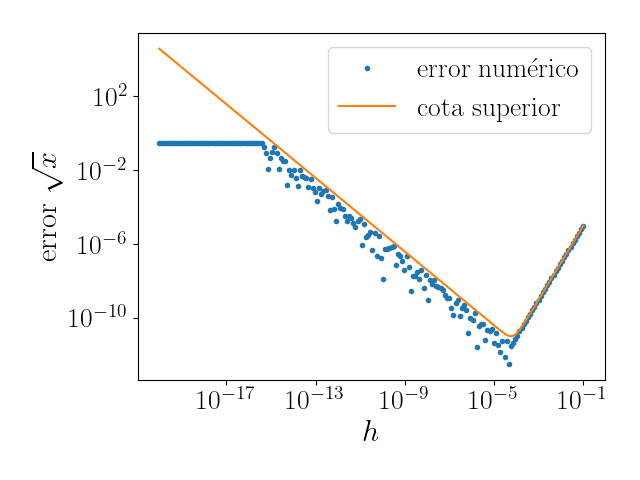
\includegraphics[width=0.8\textwidth]{ejemplo-derivada-numerica}
  \caption{Error absoluto según la ecuación~\eqref{eq:def-err-abs} con puntos azules, y \eqref{eq:err-abs-cent} con línea continua.}
  \label{fig:ejemplo_derivada_numerica}
\end{figure}

\section*{Conclusiones}
En esta actividad, analizamos el error de un esquema numérico centrado para la derivada de una función. Encontramos que el error de truncamiento es del orden $O(h^2)$, y que el error de redondeo aumenta cuando $h^2$ es muy pequeño. La cota combinada que obtuvimos muestra que hay un valor óptimo de hh donde el error total es mínimo, lo cual fue confirmado mediante gráficos comparativos.

Esta actividad me permitió entender mejor cómo interactúan los errores de truncamiento y redondeo en los esquemas numéricos. Aprendí que reducir $h^2$ indefinidamente no siempre mejora los resultados, y que es necesario balancear ambos tipos de errores para lograr una mejor precisión. Visualizar estos errores en gráficos fue fundamental para comprender su comportamiento.

\section*{Agradecimientos}
Agradezco a Carolina por ayudarme a encontrar la mayoría de los horrores ortográficos que cometí en la redacción de este capítulo. Agradezco también a mi pato de hule por las intensas y fructíferas conversaciones que me ayudaron a encontrar algunos errores en mis códigos.

\end{document}
